\documentclass[12pt]{article}

\usepackage[utf8]{inputenc}
\usepackage{sfmath}
\usepackage{amsmath}
\usepackage{graphics}
\usepackage{graphicx}

\usepackage[super, sort&compress]{natbib}
\usepackage{hyperref}
\usepackage{url}

\usepackage{tikz}
\usetikzlibrary{shapes.geometric}
 
\usepackage{physics}

\usepackage{titling}
\pretitle{\begin{center}\Huge\bfseries}
\posttitle{\par\end{center}\vspace{0.5cm}}
\preauthor{\begin{center}\large}
\postauthor{\par\end{center}}
\predate{\begin{center}\large}
\postdate{\par\end{center}}

\usepackage{geometry}
\geometry{a4paper, margin=1in}

\title{
    Mechatronics and Making \\
    Mid-Term Project Report \\
    Exoskeleton Robotic Hand With Wolf Claw Mechanism
}


\author{
    \begin{align*}
        \text{Bryan Li}\ &-  \text{SN 25003743} \\
        \text{Yan Pei Zhu}\ &-  \text{SN 25103352}\\
        \text{Nolan Yu}\ &-  \text{SN 25113715}
    \end{align*}
}

\date{October 31, 2025}

\setlength{\parindent}{0pt}
\setlength{\parskip}{1em}
\begin{document}

\begin{titlepage}
	\maketitle
\end{titlepage}

\tableofcontents

\pagebreak

\section{Introduction}
\subsection{Project Objectives and Description}
\subsection{Similar Mechanisms}
\subsection{Industrial Applications}

\pagebreak
\section{Mechanical and Mechanism Analysis}

\subsection{Drive Method and Transmission}
This robotic hand exoskeleton uses an acceleration-based machinery system.
Therefore, the movements of the finger will be amplified by this mechanism.

This mechanism can do that through a planetary gear mechanism,
whereas a belt system and a string transmission system are also needed.

Details of the transmission process shows below:

\begin{center}

	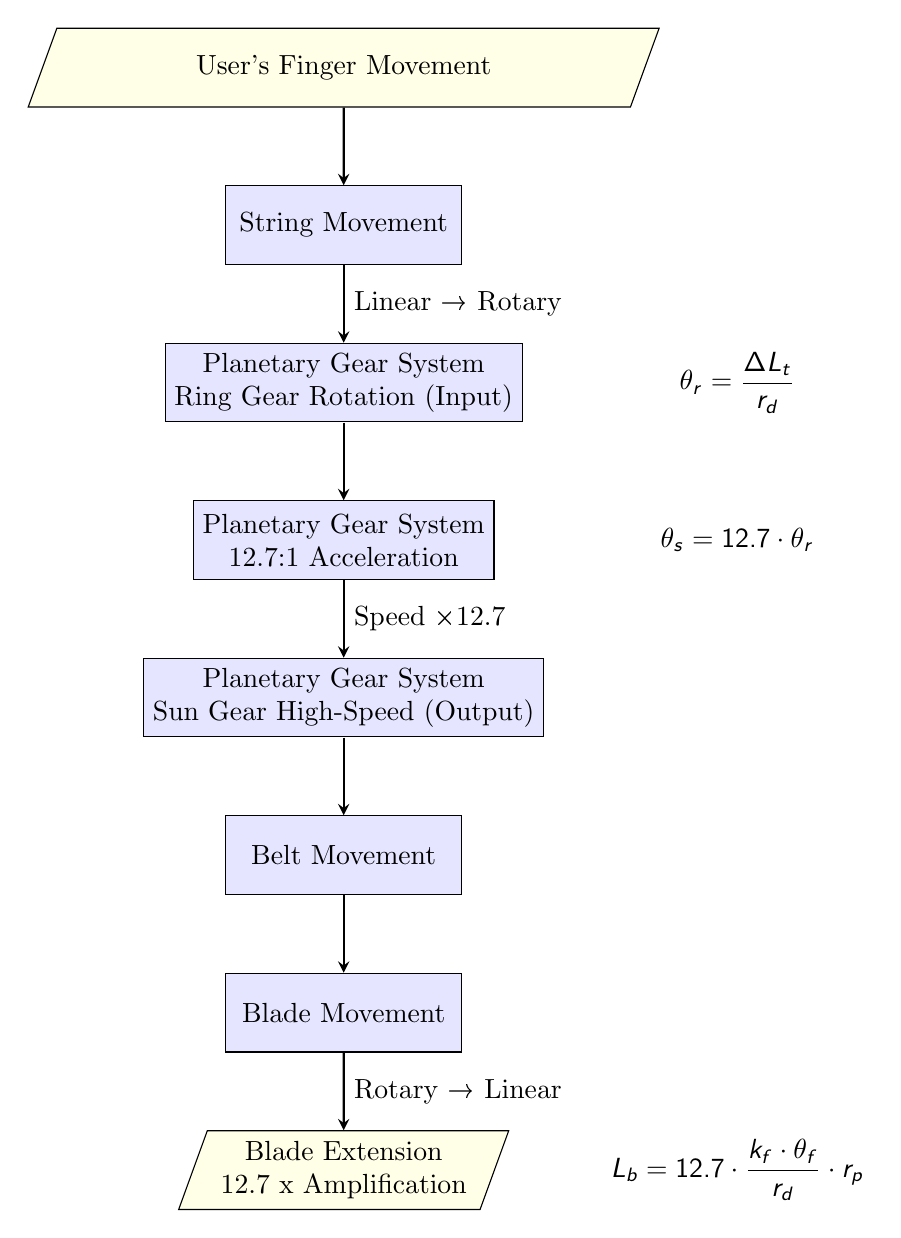
\begin{tikzpicture}[scale=0.8]

		% Define styles
		\tikzstyle{process} = [
		rectangle, minimum width=3cm, minimum height=1cm,
		text centered, draw=black, fill=blue!10, align=center]
		\tikzstyle{io} = [
		trapezium, trapezium left angle=70,
		trapezium right angle=110, minimum width=3cm,
		minimum height=1cm, text centered, draw=black,
		fill=yellow!10, align=center]
		\tikzstyle{arrow} = [thick,->,>=stealth]

		% Nodes
		\node (start) [io] {User's Finger Movement};

		\node (tendon) [process, below of=start, yshift=-1cm] {String Movement};

		\node (ring) [process, below of=tendon, yshift=-1cm] {
			Planetary Gear System \\
			Ring Gear Rotation (Input)
		};

		\node (planetary) [process, below of=ring, yshift=-1cm] {
			Planetary Gear System \\
			12.7:1 Acceleration
		};

		\node (sun) [process, below of=planetary, yshift=-1cm] {
			Planetary Gear System \\
			Sun Gear High-Speed (Output)
		};

		\node (pulley) [process, below of=sun, yshift=-1cm] {Belt Movement};

		\node (belt) [process, below of=pulley, yshift=-1cm] {Blade Movement};

		\node (blade) [io, below of=belt, yshift=-1cm] {
			Blade Extension \\
			12.7 x Amplification
		};


		% Arrows
		\draw [arrow] (start) -- (tendon);
		\draw [arrow] (tendon) -- node[right] {Linear → Rotary} (ring);
		\draw [arrow] (ring) -- (planetary);
		\draw [arrow] (planetary) -- node[right] {Speed ×12.7} (sun);
		\draw [arrow] (sun) -- (pulley);
		\draw [arrow] (pulley) -- (belt);
		\draw [arrow] (belt) -- node[right] {Rotary → Linear} (blade);

		% Kinematic equations
		\node (eq1) [right of=ring, xshift=4cm] {
			$\theta_r = \dfrac{\Delta L_t}{r_d}$
		};
		\node (eq2) [right of=planetary, xshift=4cm] {
			$\theta_s = 12.7 \cdot \theta_r$
		};
		\node (eq3) [right of=blade, xshift=4cm] {
			$L_b = 12.7 \cdot \dfrac{k_f \cdot \theta_f}{r_d} \cdot r_p$
		};
	\end{tikzpicture}

\end{center}

\pagebreak
\subsubsection{Transmission Process Details}

\textbf{User's Input (Finger Movement)}

The linear movement of the string that is deployed over the finger is created by the finger's flexion.
\begin{figure}[htbp]
	\centering
	\includegraphics[width=0.5\textwidth]{example-image}
	\caption{figure exoskeleton design}
	\label{fig:robotic figure}
\end{figure}

Total displacement of the string overhead by calculation:

\begin{equation*}
	r = 0
	P = 0
\end{equation*}

\hrule

\textbf{Biomechanical Input (Finger Flexion):}
Natural finger flexion creates geometric displacement through
overhead tendon routing on the finger dorsal side.

Using Smith et al's tendon displacement equation:

\begin{equation}
	\Delta L_t = k_f \cdot \theta_f
\end{equation}
and substituting typical finger geometry data ($k_f = 0.8$ mm/degree for index finger), we then get approximately 24 mm tendon displacement for 30 degrees of flexion. Finally, this linear displacement provides the input to the transmission system.

\textbf{Tendon to Rotary Conversion:}
The tendon wraps around a drum connected to the ring gear, converting linear displacement to rotational input. Using the drum conversion equation:
\begin{equation}
	\theta_r = \dfrac{\Delta L_t}{r_d}
\end{equation}
and substituting our drum radius ($r_d = 5$ mm) and previous tendon displacement (24 mm), we then get 4.8 radians of ring gear rotation. Finally, this rotational input drives the planetary gear system.

\textbf{Planetary Gear Acceleration:}
The ring gear serves as input in an unconventional configuration where planet gears transfer motion to the sun gear. Using the planetary gear ratio equation:
\begin{equation}
	\theta_s = 12.66 \cdot \theta_r
\end{equation}
and substituting our ring gear rotation (4.8 radians), we then get 60.77 radians of sun gear rotation. Finally, this represents the 12.66:1 acceleration that enables significant blade extension.

\textbf{Pulley and Belt Transmission:}
The sun gear shaft drives dual synchronized pulleys with timing belts maintaining parallel blade alignment. Three blades are mounted perpendicular between the belts. Using the pulley-belt transmission relationship, the rotational motion is converted to linear blade movement with the pulley radius ($r_p = 3$ mm) determining the final extension.

\textbf{Final Blade Deployment:}
Belt movement translates to linear blade extension through the complete kinematic chain. Using the comprehensive deployment equation:
\begin{equation}
	L_b = 12.66 \cdot \dfrac{k_f \cdot \theta_f}{r_d} \cdot r_p
\end{equation}
and substituting all our parameters ($k_f = 0.8$, $\theta_f = 30^\circ$, $r_d = 5$ mm, $r_p = 3$ mm), we then get 182.3 mm total blade extension. Finally, this demonstrates how subtle finger movements (30°) result in significant tool deployment (182 mm).

The complete transmission system achieves:
\begin{equation}
	\text{Overall Ratio} = \underbrace{\frac{k_f}{r_d}}_{\text{Tendon}} \times \underbrace{12.7}_{\text{Planetary}} \times \underbrace{r_p}_{\text{Pulley}} = 12.7 \cdot \frac{k_f \cdot r_p}{r_d}
\end{equation}

Where small finger movements ($\theta_f$) result in proportionally larger blade extensions ($L_b$), making the system both responsive and precise for its intended applications.


This acceleration-based transmission represents an innovative approach to
exoskeleton tool deployment, leveraging planetary gear mechanics to amplify
natural human movements into effective tool operations.
\subsection{Fingers and Wrist Mechanisms}
\subsection{Wolf Claw Mechanism Comparison}
\subsubsection{Version 1: Planetary Gear}
\subsubsection{Version 2: Compound Gear Train}


\pagebreak
\section{Mathematical Modelling and Analysis}
\subsection{Fingers and Wrist Modelling}
\subsection{Wolf Claw Mechanism \- Version 1: Planetary Gear}
\subsection{Wolf Claw Mechanism \- Version 2: Compound Gear Train}

\pagebreak
\section{Conclusion and Future Work}

\pagebreak

\bibliographystyle{plain}
\bibliography{references}

\end{document}
